\section{Engineering Dynamics Notes}

People of historic significance to the field:
\begin{itemize}
\item Copernicus 1500 (earth revolves around sun)
\item Brahe 1600
\item Kepler 1609
\item Galileo 1610 - 1620
\item Descartes 1630 1644 (kinematics) use kinematics to get to the direct method to get to the equation of motion
\item Newton 1643 1727 (3 laws 1666)
\item Euler 1707 - 1783 (angular momentum) $\mathbf H, \mathbf T = \frac{dH}{dt}$
\item Lagrange 1788 energy, work -> equations of motion
\end{itemize}

\begin{tikzpicture}
  \pgfmathsetmacro{\top}{3};
\pgfmathsetmacro{\groundres}{0.1};
\pgfmathsetmacro{\groundlen}{2};
\pgfmathsetmacro{\boxcenterline}{1};
\pgfmathsetmacro{\boxheight}{0.5}

% ground pattern
\fill [pattern = north east lines] (0,\top) rectangle (\groundlen,\top+\groundres);

% ground line
\draw[thick] (0,\top) -- (\groundlen,\top);

% spring
\draw[decoration={aspect=0.3, segment length=1mm, amplitude=1mm,coil},decorate]
  (\groundlen/3, \top) to
  node[left] {K}
  (\groundlen/3, \boxcenterline + \boxheight/2);

\draw
  (\groundlen*2/3, \top) to
  node[right] {b}
  (\groundlen*2/3, \boxcenterline + \boxheight/2);

\draw (\groundlen/4, \boxcenterline + \boxheight/2)
  rectangle (\groundlen*3/4, \boxcenterline - \boxheight/2)
  node [pos=0.5] {M};

\draw [<->] (\groundlen*5/4, 0) node[below] {y}
  to (\groundlen*5/4, \top) node[above,left] {O}
  to (\groundlen*5/4 + \top, \top) node[right] {x};

\end{tikzpicture}


\begin{itemize}
  \item Describe the motion: establish a coordinate system. $x$ from $0$ springforce position
  \item Apply physical laws: $\sum F_{external} = mx$
\end{itemize}    

\begin{itemize}
  \item draw forces in direction in which they act
  \item assume positive values for $x$, $\dot{x}$
  \item deduce signs from direction of arrows
      $f_s = x$
      $f_d = b\dot{x}$
\end{itemize}

$\sum_x F = -f_s - f_d + m_g = -Kx - b\dot{x} + m_g = m\ddot{x}$ 

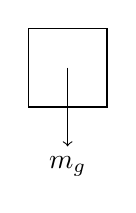
\begin{tikzpicture}
  \pgfmathsetmacro{\boxheight}{1};

\draw (0, 0) rectangle (\boxheight, \boxheight);
\draw[->] (\boxheight/2, \boxheight/2) to (\boxheight/2, -\boxheight/2) node[below] {$m_g$};

\end{tikzpicture}

$E = KE + PE = \frac{1}{2}Kx^2+\frac{1}{2}m\dot{x}^2-m_g x$

$\frac{dE}{dt}$ should be zero, since energy in system should be constant.

$Kx\dot{x} + m\dot{x}\ddot{x} - m_g\dot{x} = 0$

$m\ddot{x} =  Kx = m_g$

\subsection{Kinematics: Reference Frame and Vectors}

Notation: vector $\mathbf r_{A/O}$ is the vector originating at point $O$,
towards point $A$.

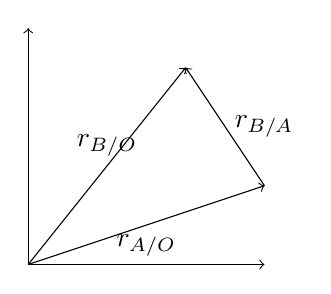
\begin{tikzpicture}
\pgfmathsetmacro{\axlen}{3};
  \coordinate (A) at (3, 1);
  \coordinate (B) at (2, 2.5);
  \draw [<->] (0, \axlen) to (0, 0) to (\axlen, 0);
  %\fill (A) circle[radius=\axlen/30] node[right] {$A$};
  %\fill (B) circle[radius=\axlen/30] node[right] {$B$};
  \draw [->] (0, 0) to node[midway,below] {$r_{A/O}$} (A);
  \draw [->] (0, 0) to node[midway,above] {$r_{B/O}$} (B);
  \draw [->] (A) to node[midway,right] {$r_{B/A}$} (B);
\end{tikzpicture}

Assume $r_{B/O} = r_{A/O} + r_{B/A}$

Derrivative of distance over time is velocity.

$\frac{d\mathbf r_{B/O}}{dt} = v_{B/O} = v_{A/O} + v_{B/A}$

Derrivative of velocity over time is acceleration.
$\frac{d^2 \mathbf r_{B/O}}{dt^2} = a_{A/O} + a_{B/A}$

Vector notes:

$\frac{d(\mathbf a + b)}{dt} = \frac{d\mathbf a}{dt} + \frac{d \mathbf b}{dt}b$

$d(f(t)\mathbf a) = \frac{df}{dt}\mathbf  a + \frac{d\mathbf a}{dt}\cdot f$

$\mathbf r_{B/O} = r_{Bx}\hat I + r_{By}\hat J + r_{Bz}\hat K$

$v_{B/O} = \frac{d}{dt}\mathbf r_{B/O} = \dot{r_{Bx}}\hat I +  \dot{r_{By}}\hat J +  \dot{r_{Bz}}\hat K$

where $\hat I$, $\hat J$, $\hat K$ are unit vectors in a fixed reference frame.

$\mathbf a_{B/O} = \frac{d}{dt} \mathbf v_{B/O} = \ddot{r}_{b_x} I + \ddot{r}_{By} J + \ddot{r}_{Bz} K$
